\section{Experimental Design}
SmallCNN has five convolutional layers, batch normalization, rectified linear activations, max pooling, dropout, and a ten-class output layer. The width-32 configuration has 160,234 parameters. We used the standard CIFAR-10 split of 50,000 training and 10,000 test images~\cite{cifar10}. Training images were randomly cropped with four pixels of padding and randomly flipped horizontally. Test images were normalized without augmentation. The watermark training recipe used 30 epochs, batches of 128, Nesterov stochastic gradient descent with momentum 0.9, weight decay $5\times10^{-4}$, and a cosine schedule starting at 0.05. The main comparisons use $\lambda=20$ and hinge margin $m=1.5$~\cite{projectResults}.

Baseline, BCE/RS32, and hinge/RS32 accuracy comparisons use seeds 0--4. BCE/RS16 uses seeds 0--2; its accuracy cost is paired with those same baseline seeds. Robustness evaluations use seeds 0--2 for all three designs. Each design contributes 252 checkpoint evaluations including clean controls and repeated random modifications. The suite covers noise, pruning, quantization, fine-tuning, channel permutation and scaling, and watermark overwrite. A successful removal requires \textsc{Rejected} and a test accuracy drop of at most five percentage points relative to that seed's clean watermarked model. All reported counts use the saved checkpoint verdicts~\cite{projectResults}.

\section{Results}
\subsection{Accuracy and watermark strength}
Mean test accuracy was 84.60\% for the baseline, 82.37\% for BCE/RS32, and 84.10\% for hinge/RS32. Hinge improved accuracy over BCE on each of the five paired seeds (Fig.~\ref{fig:accuracy}). Across paired seeds the gain ranged from 0.92 to 2.40 percentage points, with a mean of 1.73. Relative to the unwatermarked baseline, the mean paired accuracy changes were $-2.23$ points for BCE/RS32 and $-0.50$ for hinge/RS32 (sample standard deviations 2.18 and 1.79 points, respectively). BCE/RS16 achieved 82.26\% across its three seeds, a paired cost of 2.81 points. All three designs recovered the clean payload without decoded bit errors.
\begin{figure}[!tb]
\centering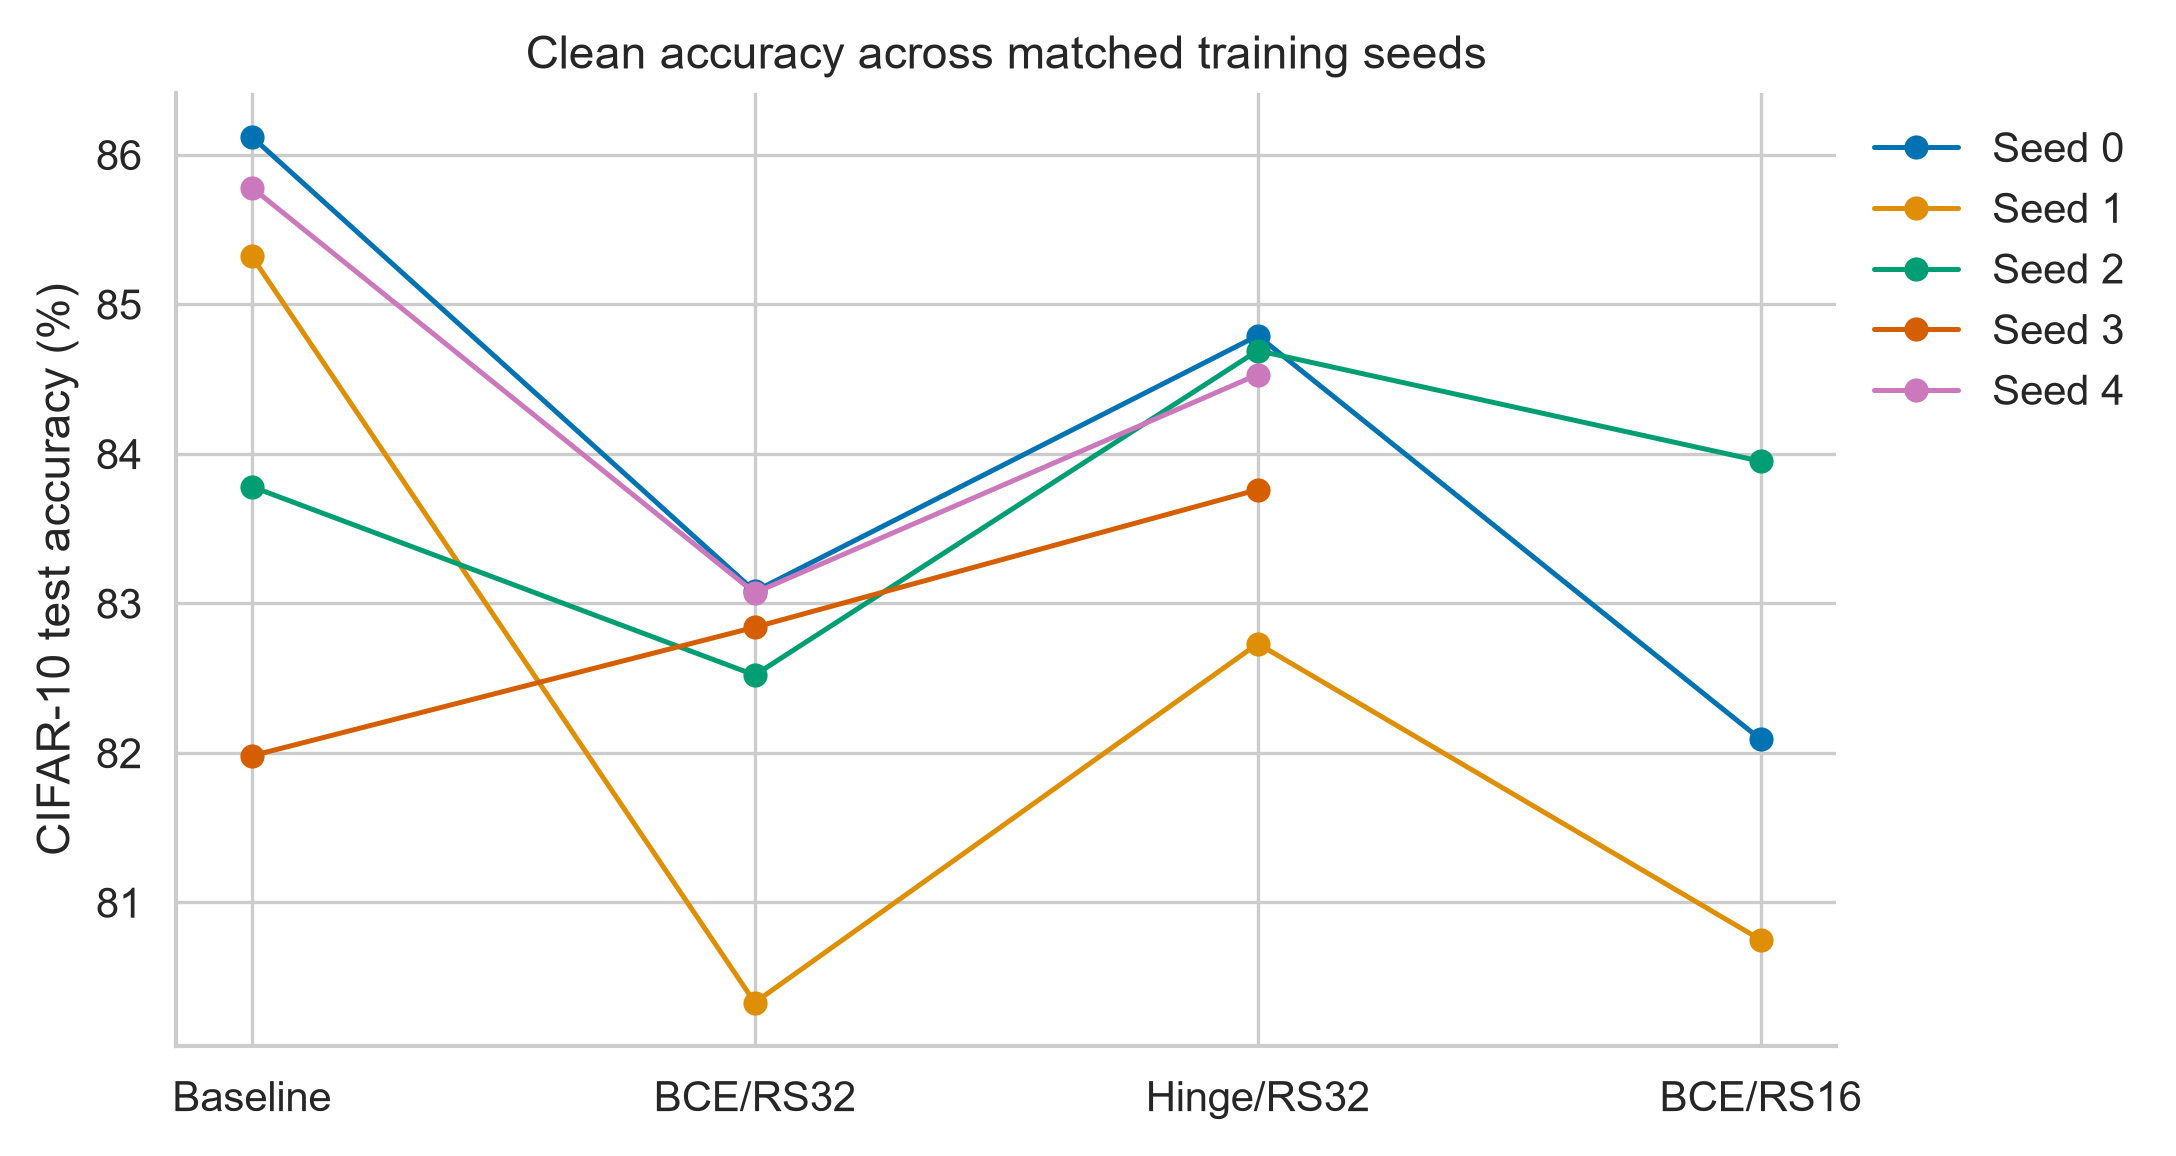
\includegraphics[width=\columnwidth]{figures/01_paired_accuracy.png}
\caption{Clean CIFAR-10 accuracy. Lines connect runs sharing a training seed. RS16 has three paired seeds.}\label{fig:accuracy}
\end{figure}

The available matched strength comparison covers seed 0. Increasing $\lambda$ from 1 to 5 to 20 raised the minimum absolute projection score from 0.02 to 1.21 to 2.25. Accuracy declined from 84.67\% to 83.19\% to 83.08\% (Fig.~\ref{fig:strength}). The margin measures how close the weakest bit lies to the decoding boundary before modification. Its increase alone does not establish resistance to overwrite.
\begin{figure}[!tb]
\centering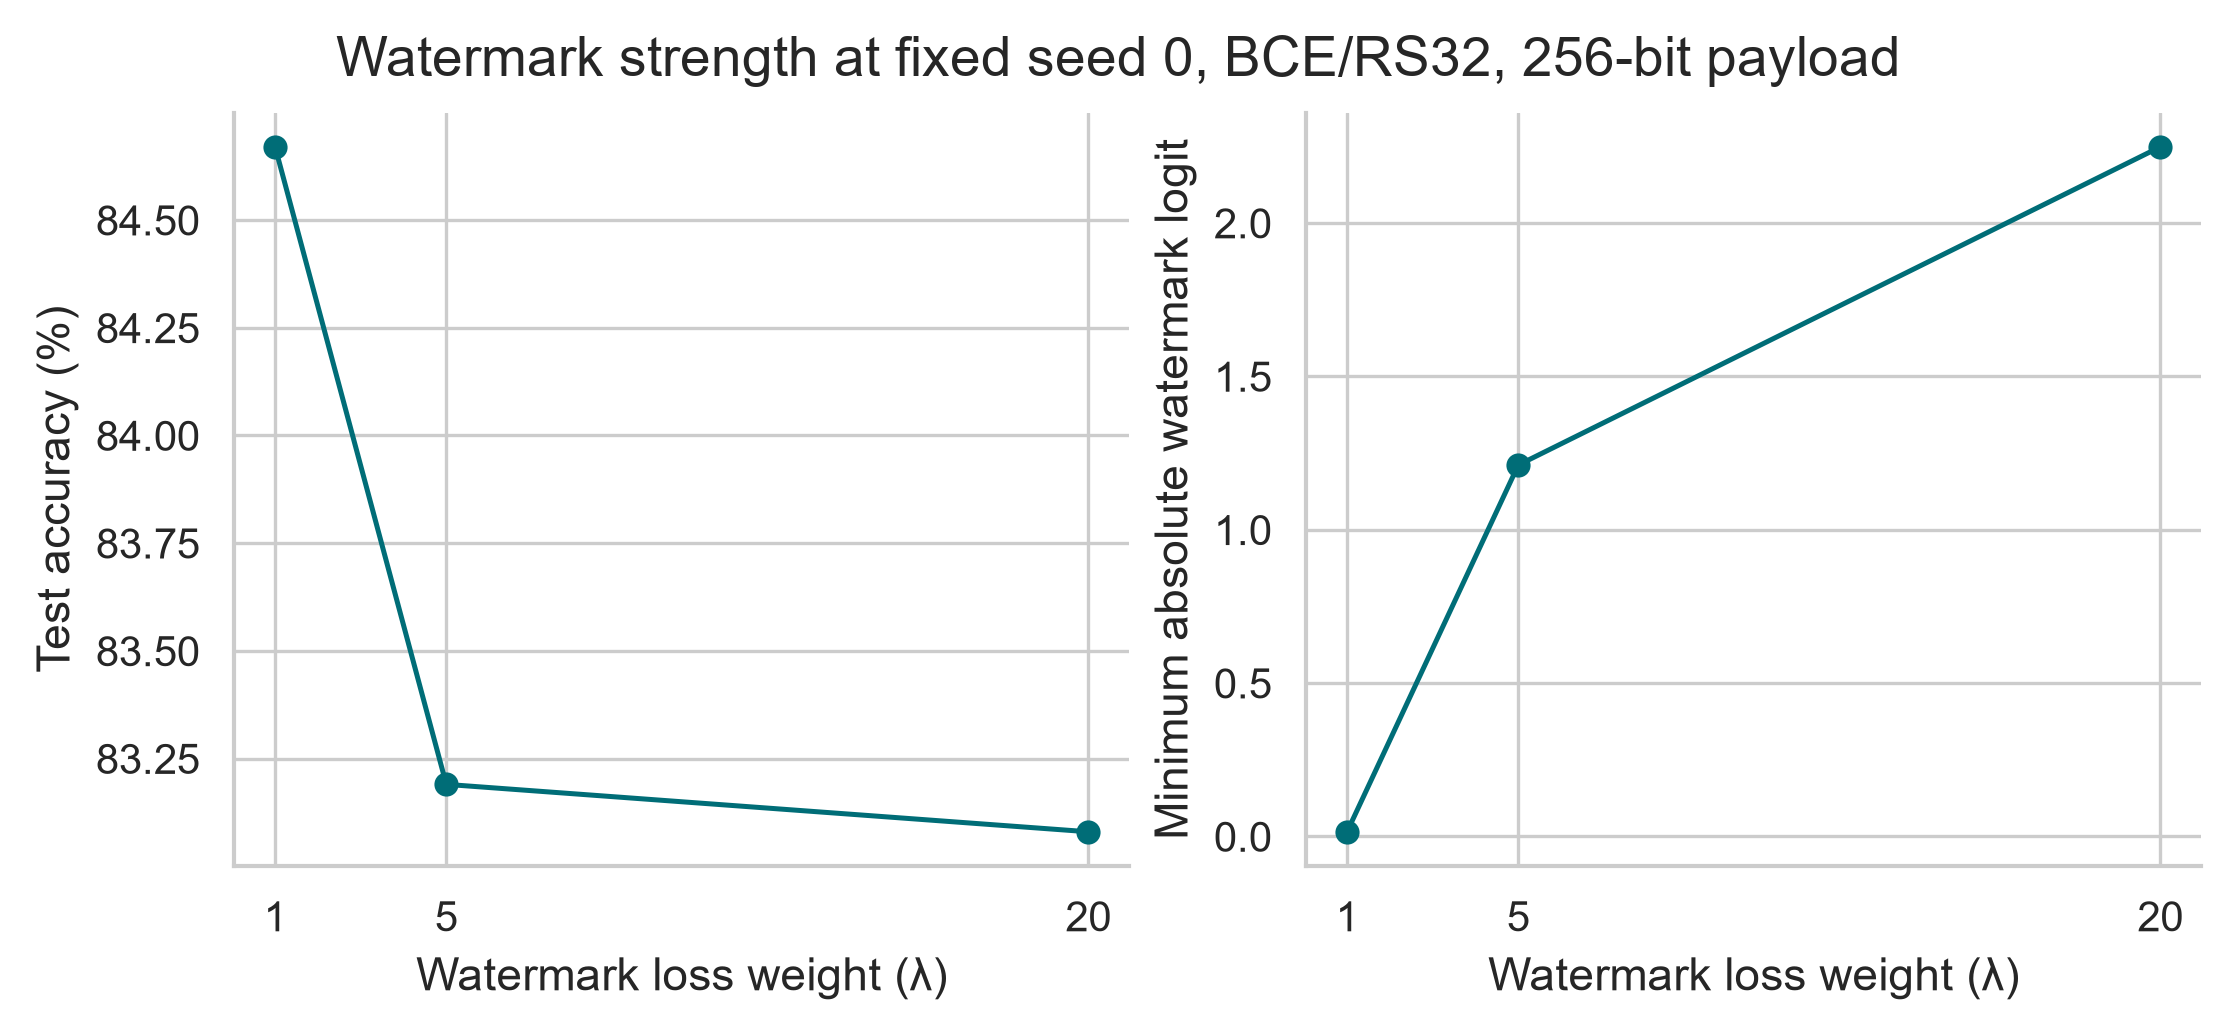
\includegraphics[width=\columnwidth]{figures/03_strength_seed0.png}
\caption{Effect of watermark strength at fixed seed, carrier layer, loss and payload. Each point represents one training run.}\label{fig:strength}
\end{figure}

\subsection{Robustness at comparable utility}
Of the 252 BCE/RS32 checkpoints, 231 verified exactly, 20 retained sufficient evidence for a damaged verdict, and one was rejected. That rejection occurred after 2-bit quantization with a large accuracy loss. BCE/RS16 yielded 240 exact and 12 damaged verdicts. Neither BCE configuration had a successful removal within the utility limit. All 108 evaluations involving channel permutation, including combined permutation and scaling, verified across the three designs.

Hinge/RS32 gave 233 exact, 13 damaged, and six rejected verdicts. Three rejections met the removal criterion. In each case a second 512-bit watermark was embedded in the carrier layer. Test accuracy fell by 4.71, 3.38, and 4.48 points for seeds 0, 1, and 2, respectively (Fig.~\ref{fig:robust}). Counting only exact recoveries would rank hinge slightly ahead of BCE/RS32 and conceal this difference. Conditioning rejection on retained model utility identifies the vulnerability.
\begin{figure*}[!t]
\centering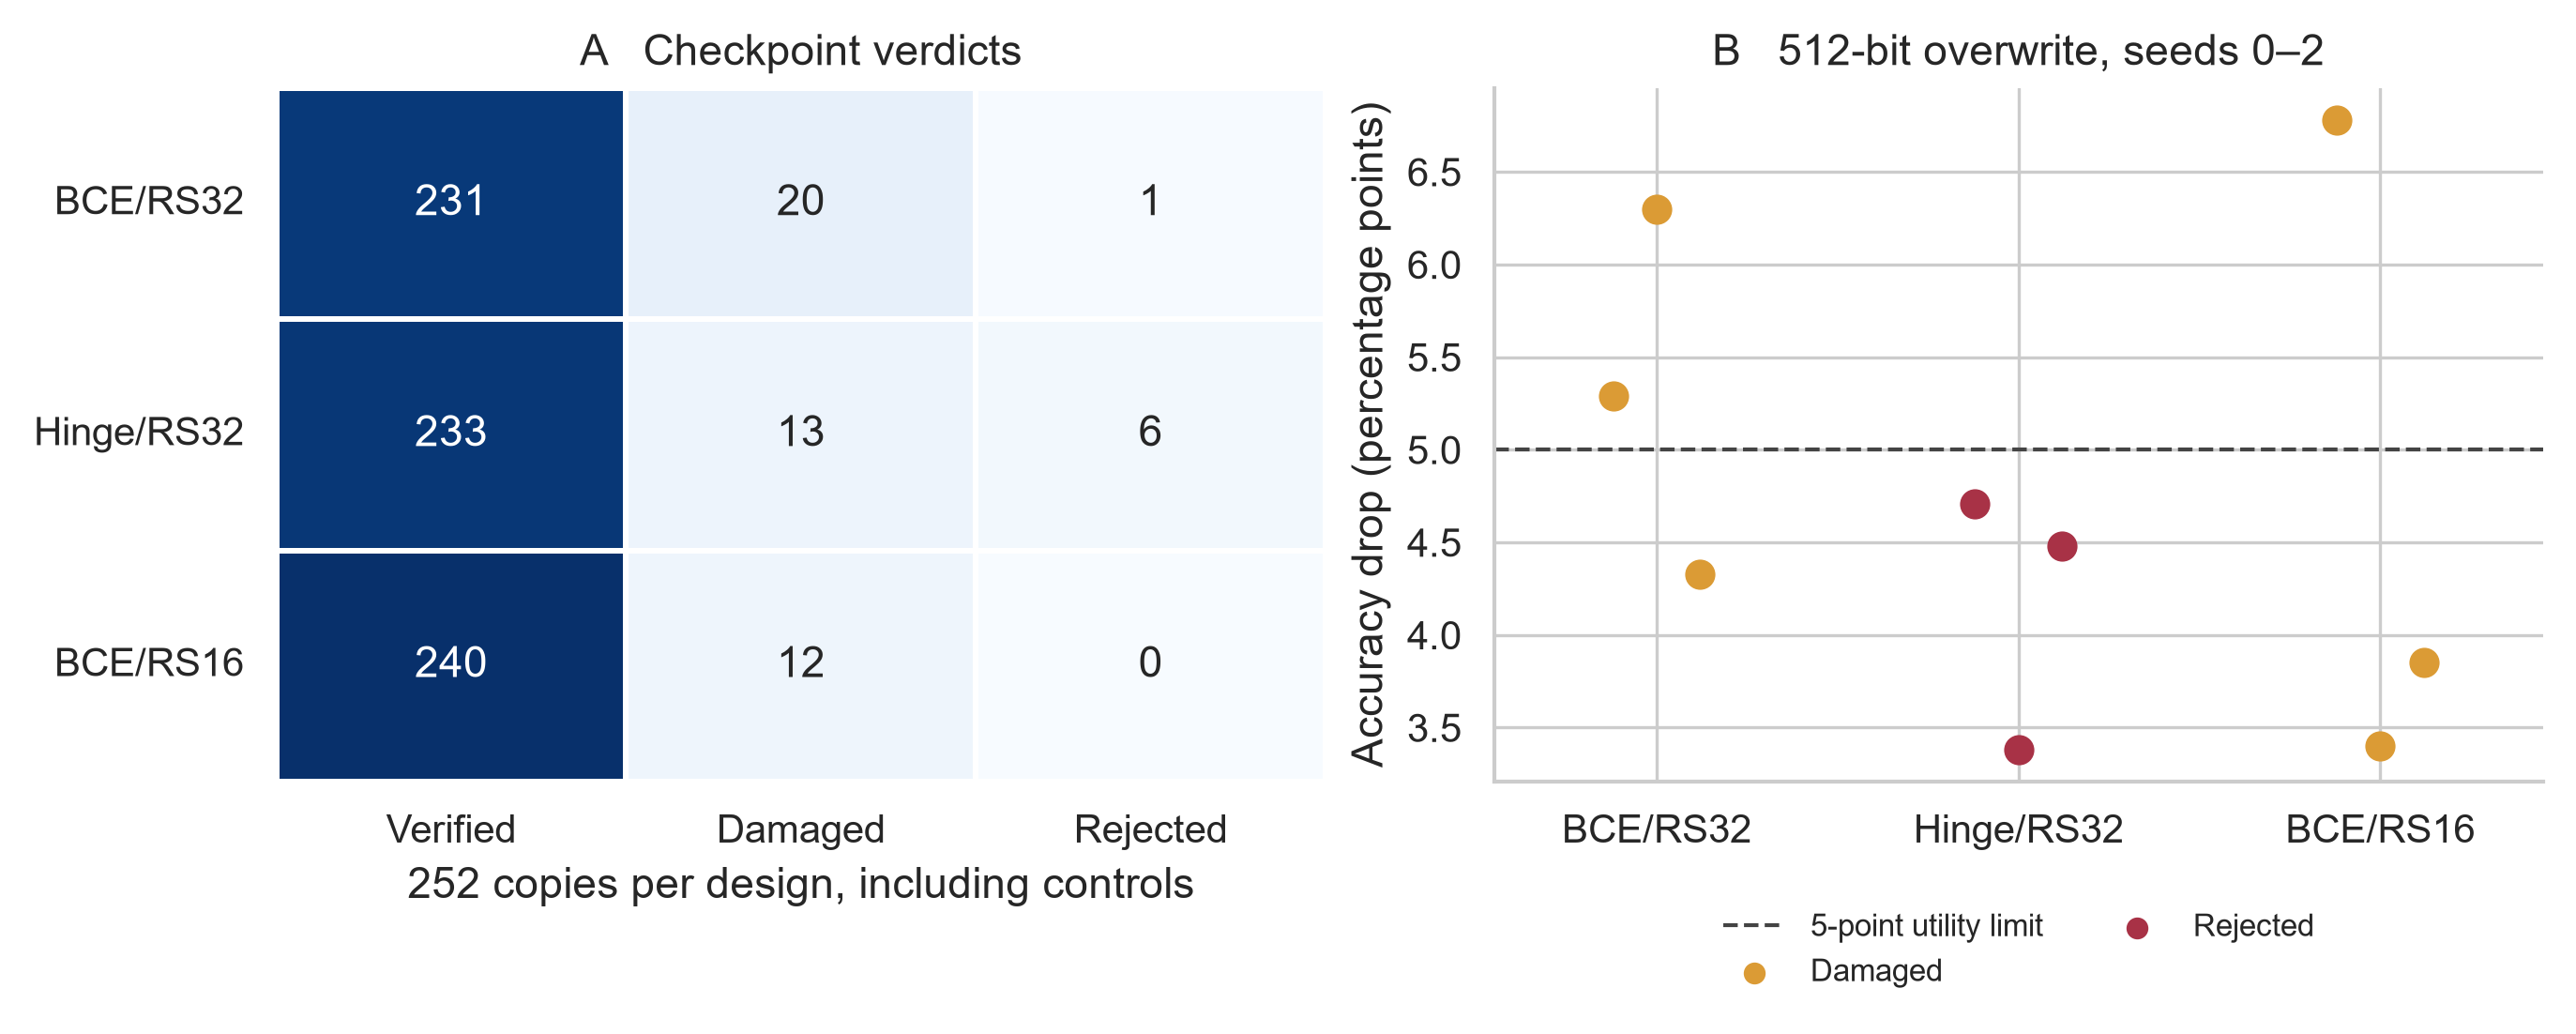
\includegraphics[width=0.91\textwidth]{figures/02_robustness.png}
\caption{Left: verifier outcomes on the same suite for each design. Right: accuracy change and verdict for each 512-bit overwrite. A rejected copy at or below the five-point limit counts as a successful removal.}\label{fig:robust}
\end{figure*}

\subsection{Error correction and negative controls}
In the original BCE/RS32 quantization evaluation, 3-bit per-tensor quantization flipped an average of 1.1\% of raw codeword positions, yet the decoder recovered the exact payload for all three seeds (Fig.~\ref{fig:ecc}). Mean classification accuracy fell by approximately 57.6 percentage points in that condition. Payload recovery and preservation of the classifier therefore require separate measurements.
\begin{figure}[!tb]
\centering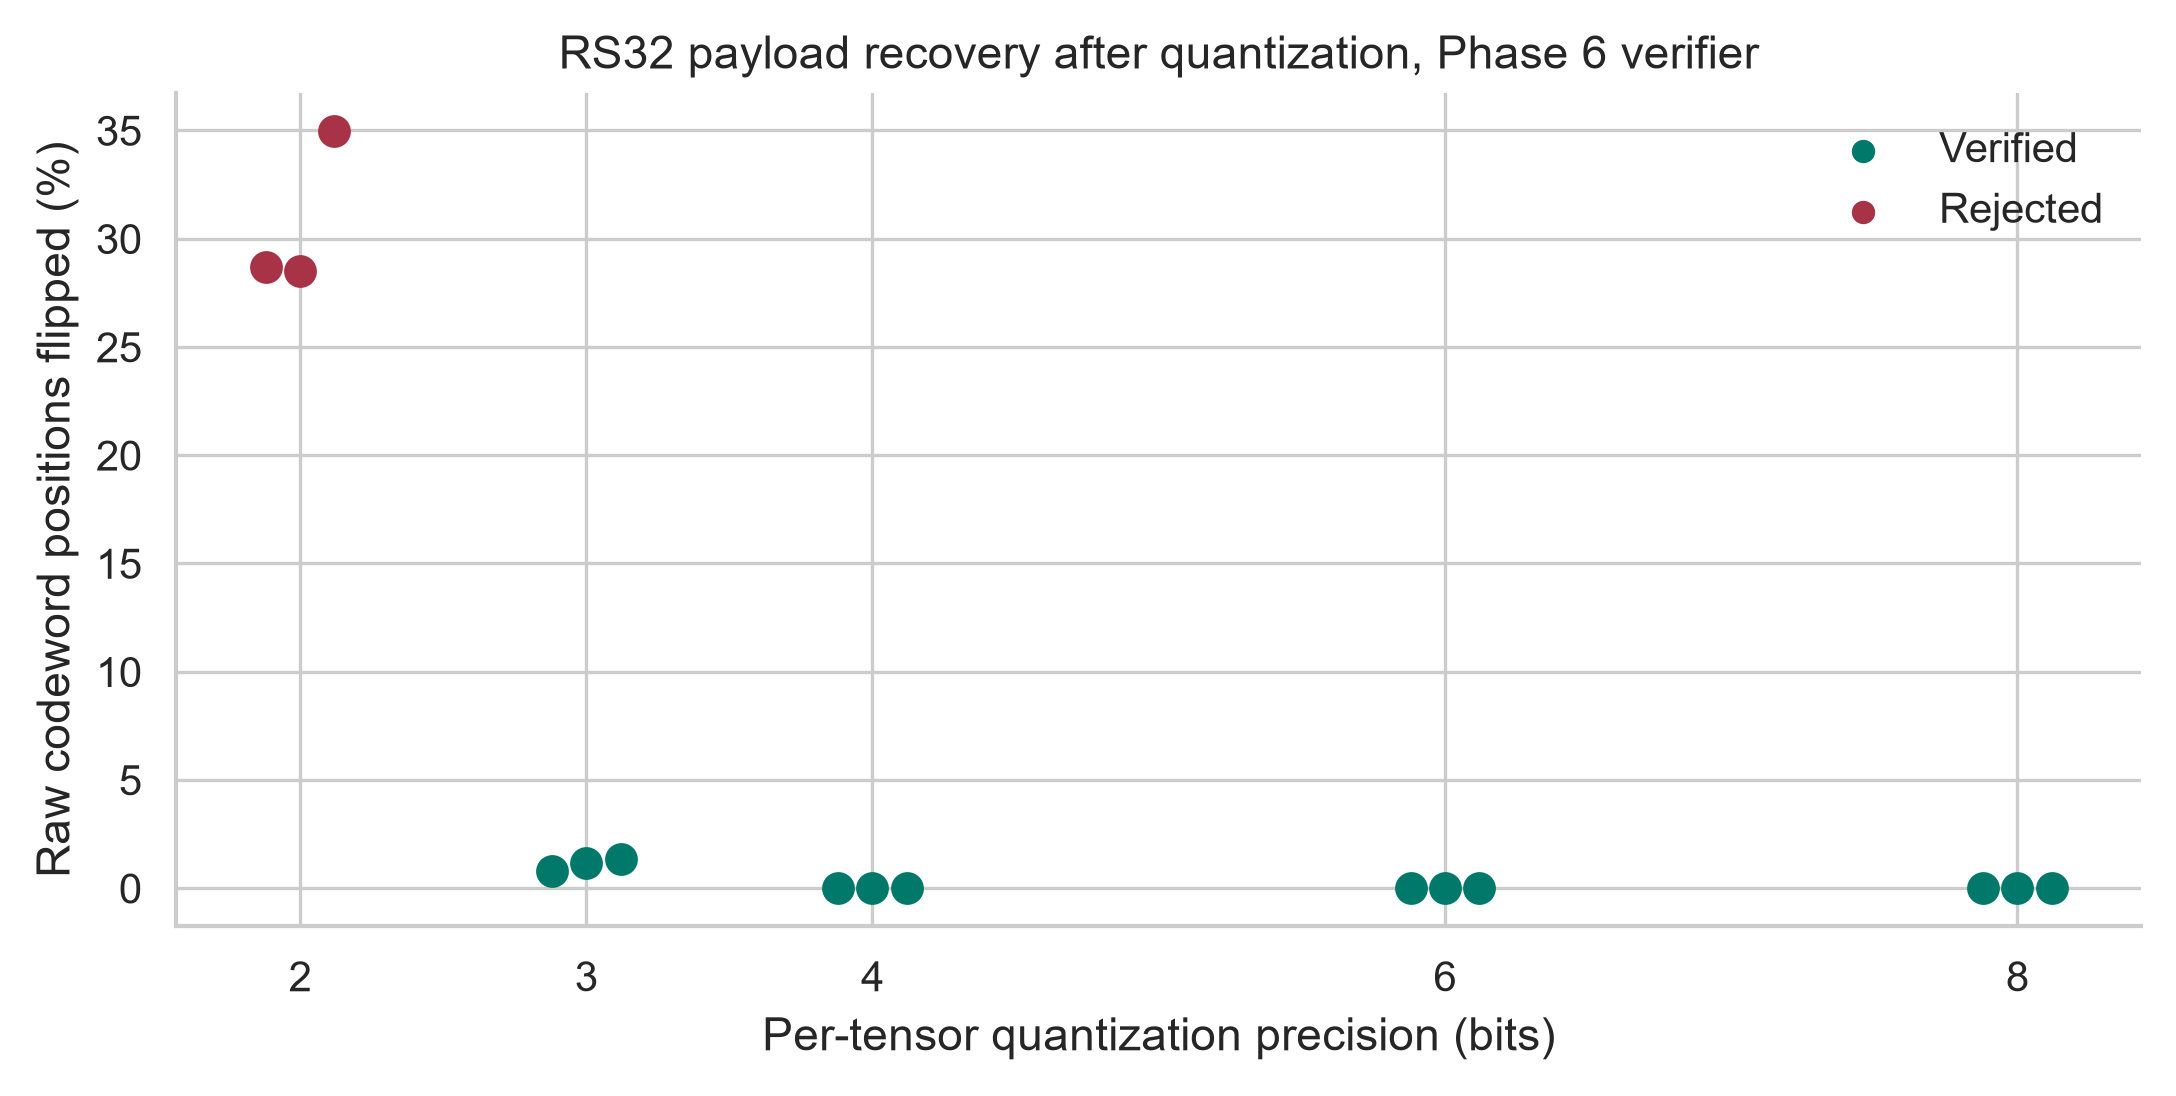
\includegraphics[width=\columnwidth]{figures/05_ecc_quantization.png}
\caption{Raw codeword errors under per-tensor quantization. Colors give the original Phase 6 verifier verdict, before the channel-alignment extension.}\label{fig:ecc}
\end{figure}

The RS32 control study comprised 724 cases, including 600 wrong-key trials and 100 random initializations. The largest raw agreement was 305 of 512 positions, below the damage threshold of 358 (Fig.~\ref{fig:null}). No case received a verified or damaged verdict. A separate set of 54 attacked baseline checkpoints also yielded zero false detections. These are empirical counts across the sampled cases; repeated trials on a shared checkpoint do not represent independently trained models.
\begin{figure}[!tb]
\centering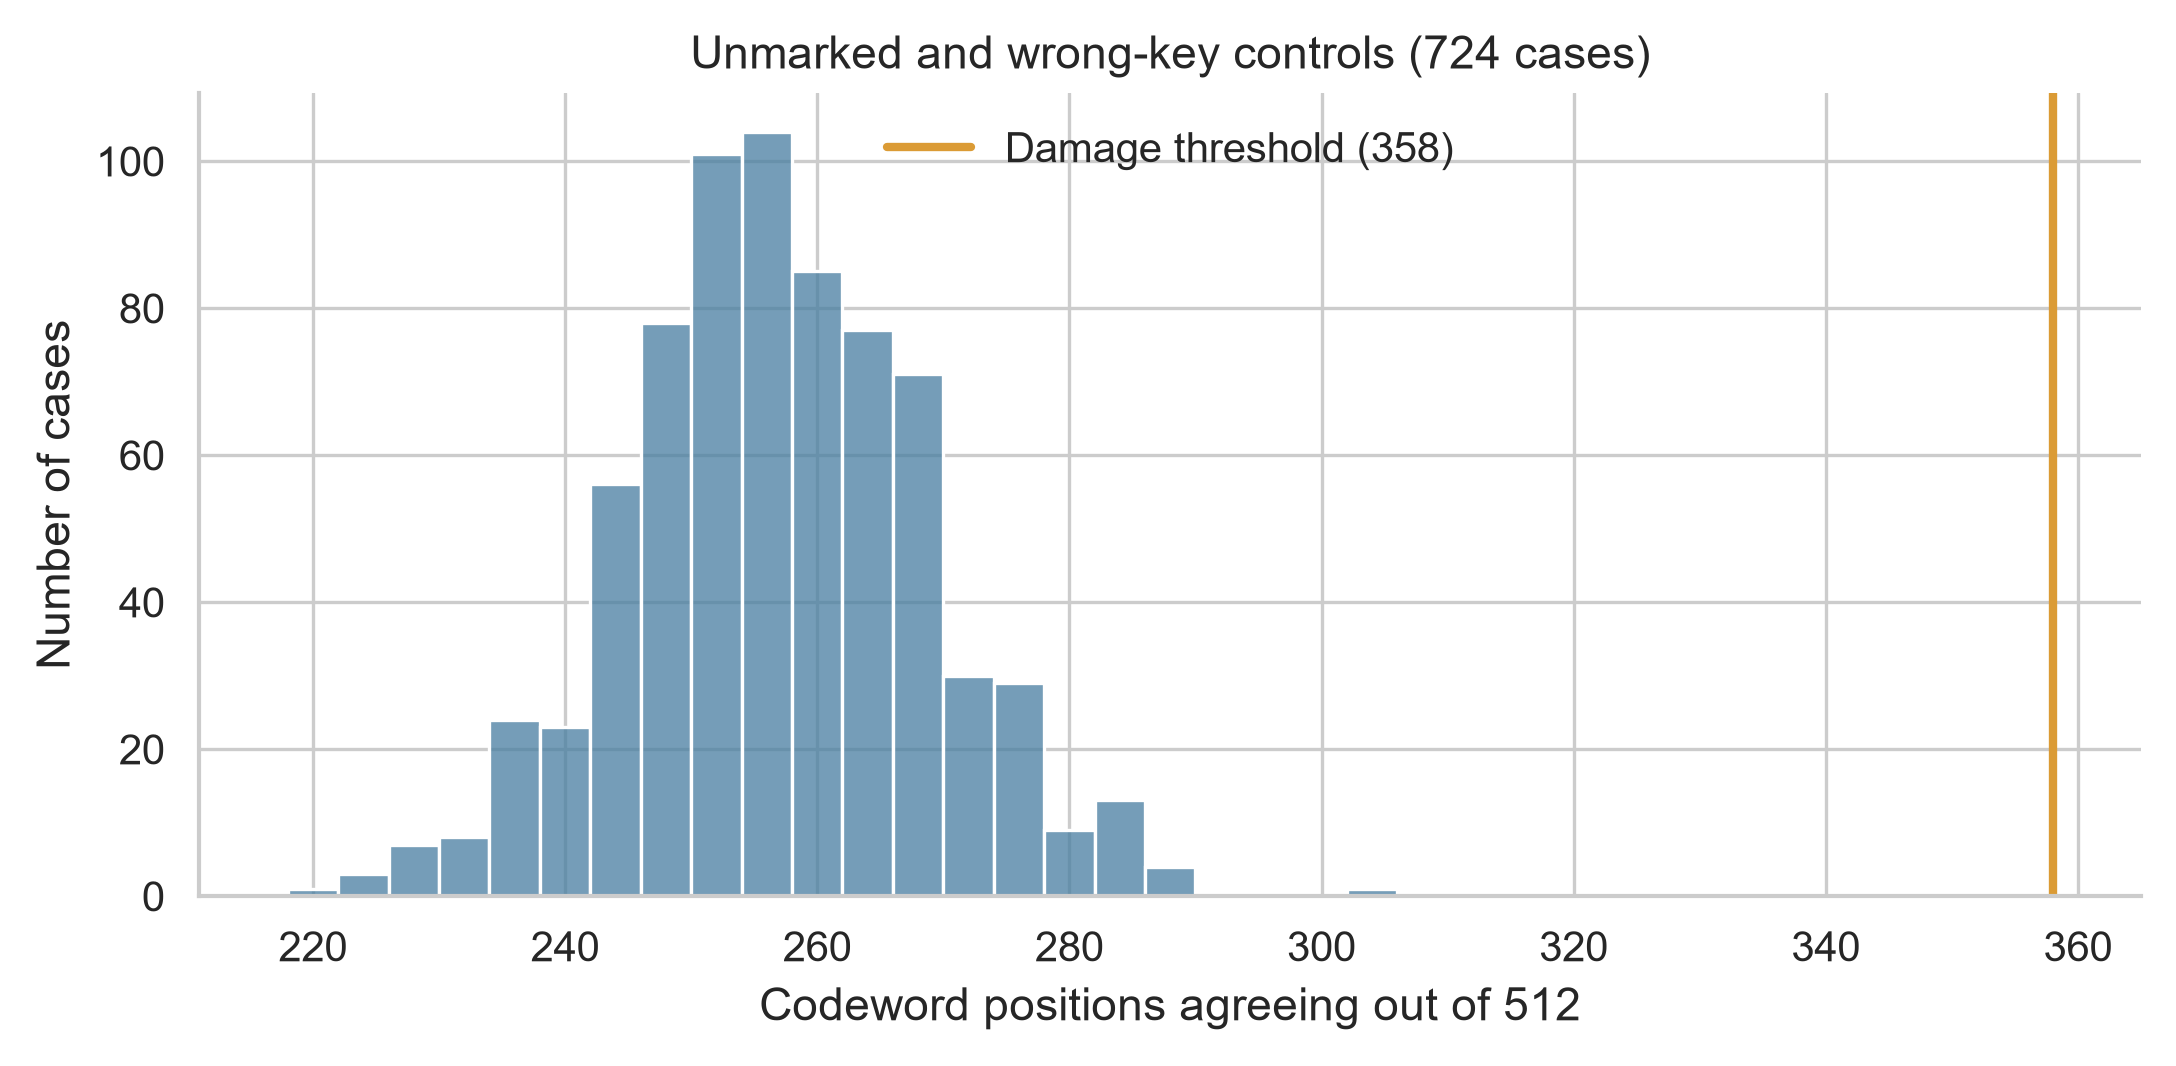
\includegraphics[width=\columnwidth]{figures/04_false_positive_controls.png}
\caption{Agreement with the signed codeword across 724 controls. The vertical line is the RS32 threshold for residual evidence.}\label{fig:null}
\end{figure}

\clearpage
\section{Discussion and Limitations}
An auxiliary comparison on two seeds assigned each code bit to the sign of a single keyed weight. This naive embedding changed clean accuracy by only $-0.09$ points on average, but six tested weight-modification configurations achieved a successful removal. The projection comparison used three seeds and more random draws per stochastic configuration. These different sample sizes limit the precision of a head-to-head rate comparison~\cite{projectResults}.

The strongest evidence for the loss comparison comes from holding architecture, code and training seed fixed. The five seed pairs establish a consistent direction for the observed accuracy change. The three overwrite trials expose a repeatable failure in this setup, but they do not yield a general removal probability. All measurements concern one classifier architecture, dataset, carrier and trusted-auditor setting. An auditor who discloses the watermark key changes the attacker's capabilities. A release intended for deployment also requires signing keys under exclusive developer control.

The current experiments do not isolate the accuracy cost of enabling error correction or varying the payload length. RS16 and RS32 both carry 256 payload bits and differ in redundancy. A matched no-code control and shorter payloads at fixed code rate remain future work. The theoretical raw-agreement threshold and the empirical controls likewise leave open a rigorous false-accept bound for the full permutation-plus-scaling search.

\section{Conclusion}
The prototype connected a signed release record to a CIFAR-10 classifier through an error-corrected weight watermark. The central result is a measured tradeoff: capping the watermark margin recovered 1.73 points of clean accuracy, while a same-layer overwrite removed the mark at useful accuracy on every tested hinge seed. Both BCE configurations resisted successful removal in the same suite, at a larger paired clean-accuracy cost. For this setting, a meaningful provenance evaluation must report the verifier's verdict and the utility of the modified classifier together.
